\section{Evaluation}
\label{section:evaluation}

Here we present the evaluation of a distributed CQBS broker.
All brokers and coordinators machines were chosen to emulate commodity hardware; for CQBS to be an effective solution, it must not rely on intractably large resources.
Hence, we chose to use the \texttt{t2.medium} AWS instance type with 2 vCPUs and 4 GB RAM, running Ubuntu 14.04.
As we will demonstrate below, the CQBS system is amenable to commodity systems because its performance is limited by the serialization of the etcd log, and not by memory, CPU, disk, or network bandwidth.

\subsection{Single-Broker Performance}

\begin{figure}[t]
\centering
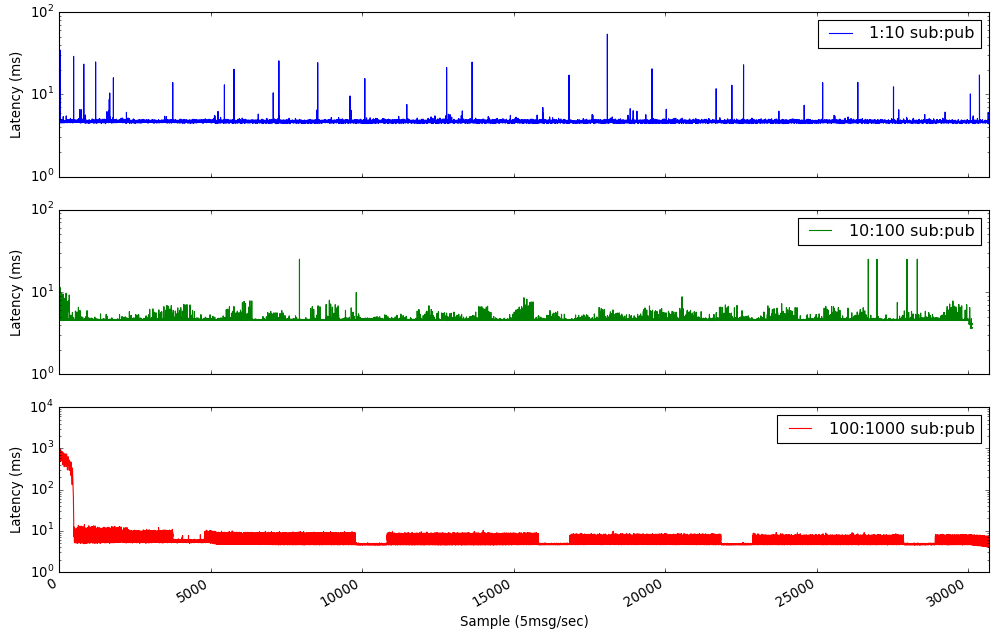
\includegraphics[width=\linewidth]{figs/singlenodelatency.png}
\caption{Microbenchmark: standalone CQBS broker forwarding latency with increasing concurrency.}
\label{fig:singlenodelatency}
\end{figure}

First, we examine the latencies of the CQBS broker's forwarding mechanism in isolation---without the communication overhead imposed by the fully replicated system.
We run a single broker on a \texttt{t2.medium} instance, backed by MongoDB\@.
Using a ratio of 10 publishers to one subscriber, we run three benchmarks with 1, 10 and 100 subscribers (with 10, 100 and 1,000 publishers accordingly).
Each publisher sends 5 messages per second; after the initial registration message (marked by the high latencies at the beginning of each benchmark), each publisher sends only its stream UUID and an increasing counter as its value.
Each group of publishers/subscribers use entirely isolated sets of keys, so that they do not explicitly interfere with each other in the broker.
These three microbenchmarks are shown in Figure~\ref{fig:singlenodelatency}, and demonstrate that the latency is fairly consistent as the amount of concurrency scales.

The spikes in latency seen in the $N=1,10$ graphs are due to the pauses enacted by Go's garbage collection.
Fortunately, these do not affect the vast majority of requests.
For the $N=1,10$ cases, the mean latencies, 95\textsuperscript{th} percentile latencies and standard deviation are $4.67ms/4.85ms/0.55ms$ and $4.62ms/4.77ms/0.37ms$ respectively.
For the $N=100$ case, the garbage collection becomes more visible in the variability of response times, with mean, 95\textsuperscript{th} percentile and standard deviation latencies of $13.58ms/8.87ms/67.13ms$.
The troughs in the $N=100$ case are an odd phenomenon, most likely caused by garbage collection in the single Go process used to generate the 100 subscribers and 1000 publishers, generating approximately 5000 messages per second.

The microbenchmark demonstrates that a single broker can quite easily handle a constant load of publishers and subscribers with low latency, even on commodity hardware.

\subsection{Coordinator Performance}

\begin{figure}[t]
\centering
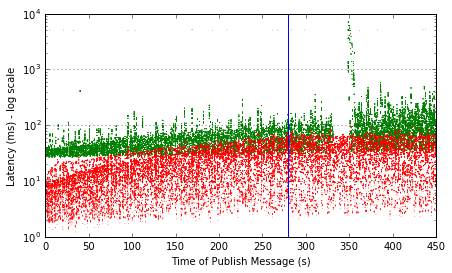
\includegraphics[width=\linewidth]{figs/coordinator_performance.png}
\caption{Microbenchmark: coordinator latency in the face of failures.
Red dots indicate running a single-node coordinator with no replication or fault tolerance; green dots indicate running a full three-node coordinator with fault tolerance via Etcd.
At the blue line at approximately 280 seconds, the system switches from adding new publishers to existing publishers changing their metadata.
At the gap seen in the replicated results at approximately 325 seconds, the leader node of the coordinator node was shut down.}
\label{fig:coordinator_performance}
\end{figure}

Next we examine the latency of the central coordinator's query evaluation and decision making processes.
We run the coordinator in two different modes; one with a single-machine coordinator which has no fault tolerance and does not use Etcd, and one with a full three-node coordinator cluster which is fully replicated via Etcd.
In both cases the coordinator nodes are run on \texttt{t2.medium} instances.
We start 10 ``dummy'' brokers which act as if they have publishers and subscribers attached to them.
These brokers load the system with a total of 500 subscribers, each of which subscribes to 10\% of the total publishers in the system at any given time.
At the start of the experiment there are no publishers in the system.
New publishers are added to the system at intervals uniformly randomly spread between 50 and 500ms, until there are a total of 1000 publishers in the system.
At this point, no new publishers enter the system, but the existing publishers start to change their metadata at the same frequency, causing the set of subscribers to which they are relevant to change over time.
We measure the latency of handling the new publisher joining the system, which is defined as the time elapsed between when the publication message is first sent to the coordinator until the time at which a subscriber receives a notification about the new publisher's presence.

In the case of the fully replicated coordinator cluster, we also force the leader of the cluster to fail, causing one of the replicas to become the new leader, and causing all brokers to have to reconnect to this new leader.

Latency results are shown in Figure~\ref{fig:coordinator_performance}; each dot represents the latency from the viewpoint of a subscriber which received a notification about a new publisher.
For the replicated and unreplicated cases respectively, the mean and 95\textsuperscript{th} latencies are $95.5ms$/$191.2ms$ and $24.7ms$/$57.3ms$.
We see that in both the replicated and unreplicated cases, latency increases as more and more publishers are added to the system (before 280 seconds), and levels off once the publishers are only changing their metadata (after 280 seconds).
We also see that the unreplicated coordinator is over an order of magnitude faster in the best cases, and the highest latencies experienced by the unreplicated coordinator are similar to the lowest latencies experienced by the replicated coordinator.
No request to the replicated coordinator takes less than 30--40ms, which is approximately the latency of an Etcd store operation in our experimental setup.
This is indicative of the fact that the serialization process through Etcd is a significant bottleneck in our system that severely limits throughput and degrades latency, and indicates that moving Etcd storage farther from the hot path of coordinator decisions could be very beneficial; this is discussed further in Section~\ref{subsec:alternate_designs}.

At approximately 325 seconds we force one of the leaders to fail.
This can be seen on the plot as a gap in latencies, since no messages could be sent during this time.
The approximately 15 seconds for brokers to reconnect is primarily due to the latency of switching over the Elastic IP address via Amazon AWS API calls, as discussed in Section~\ref{subsec:coordinator_fault_tolerance}.
The large spike in a small number of latencies immediately following is due to the fact that some brokers were able to reconnect more quickly, so they began sending messages destined for brokers which had not yet reconnected.
However, once all brokers were able to reconnect, we see that the system is able to settle back into a stable state with reasonable levels of latency.

\subsection{Full-System Performance}

\begin{figure}[t]
\centering
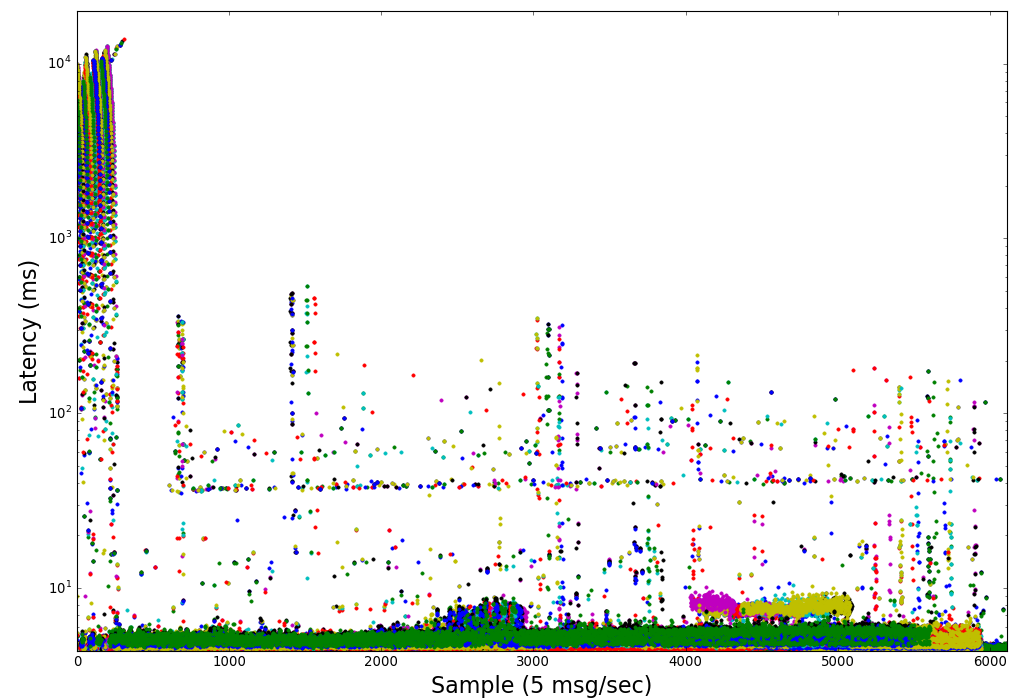
\includegraphics[width=\linewidth]{figs/fullsystem_metadatachange.png}
\caption{Benchmark: forwarding latency with 30 subscribers and 360 publishers in a 3 broker, 3 coordinator system. Each publisher changes metadata every 30--60 seconds, causing the broker to reevaluate roughly a third of all subscriptions every few seconds.}
\label{fig:fullsystem_metadatachange}
\end{figure}

To evaluate the overhead of the continuous syndication mechanism, we construct a three broker, three coordinator cluster, with every component running on a different machine.
We then introduce 10 subscribers at every broker; each subscribes to 4 local publishers (same broker) and 4 remote publishers at each of the other two brokers for a total of 12 subscriptions.
In total, there are 120 publishers per broker, with a total of 30 subscribers and 360 publishers in the benchmark.
Each publisher changes its metadata every 30--60 seconds, causing the publishers to cycle among the subscribers.
The results are illustrated in Figure~\ref{fig:fullsystem_metadatachange}, which illustrates the limitations of serializing the processing of all metadata changes and coordinator updates.
While the 95\textsuperscript{th} percentile latency is only $7.59ms$, the mean latency over the experiment was $129.60ms$ with a standard deviation of $891ms$.
This variability is caused when several metadata updates arrive at the coordinator in quick succession: the coordinator buffers these changes until it can process them sequentially, making sure that the forwarding tables are correct and consistent.
Because no related messages can be forwarded until the forwarding changes are known, a queue of metadata changes causes cascading delays until the system can catch up.
This phenomenon is most prominent around samples 800, 1500, 3000 and 4000.
The ``waterfall'' at the beginning of the stream is caused by all 30 subscribers and 360 publishers querying and registering at the same time, placing a large load on MongoDB and the etcd log.

When considered in conjunction with the microbenchmark above, it is clear that the serialization of the metadata changes and coordinator updates is the limiting factor in system performance.
However, in the authors' experience with real world sensor systems using similar systems, these high rates of change are rarely seen: it is important to note that these loads are intentionally unrealistic to find the bottlenecks in the system.

\subsection{Client Complexity}

One goal of this system was to maintain a low level of client complexity.
To evaluate this, we have written clients in the Go and Python languages.
Publishers are capable of publishing values and modifying their metadata, and subscribers are capable of submitting queries and attacking handler functions to respond to inbound published messages and notifications about changes to the set of publishers which they are currently subscribed to.
Both types of clients are capable of contacting the coordinator to seamlessly handle the failure of their local broker.

\begin{table}
\centering
\caption{Lines of non-comment, non-whitespace code used to implement programmable clients in Python and Go.
Base Code is the basic code necessary to communicate with the system, Failover is the code necessary to communicate with the coordinator to handle broker failures, and Subscriber/Publisher are the code necessary to implement subscriber- and publisher-specific functionality on top of the shared code.}
\label{tbl:client_code}
\begin{tabular}{ | c | c | c | c | c | c | }
\hline
Language & Base Code & Failover & Subscriber & Publisher & Total
\\\hline
Go & 175 & 111 & 65 & 69 & 420
\\\hline
Python & 105 & 60 & 28 & 33 & 226
\\\hline
\end{tabular}
\end{table}

We present figures for the number of lines of code necessary to create clients in both Go and Python in Table~\ref{tbl:client_code}.
The Python client was easily developed in under one day of effort, indicative of the simple nature of the communication protocol and the ease with which it could be implemented on any number of platforms and devices.
In this regard we consider ourselves highly successful, providing very high availability while managing to require extremely simple client logic.

%%% Local Variables:
%%% mode: latex
%%% TeX-master: "paper"
%%% End:
